\renewcommand{\theequation}{\theenumi}
\begin{enumerate}[label=\arabic*.,ref=\thesubsubsection.\theenumi]
\numberwithin{equation}{enumi}
%
\item Let 
%
\begin{align}
y &= 3x + 1
\implies \myvec{3 & -1}\vec{x} &= -1
\end{align}
%
Thus, 
%
\begin{align}
y &= 0 
\\
\implies  3x + 1 &=0
\\
\text{or, } x &= -\frac{1}{3}
\end{align}
%
Hence $\vec{x}=\frac{1}{3}$ is not a zero. This is verified in Fig. \ref{fig:line1}.
%
\begin{figure}[!ht]
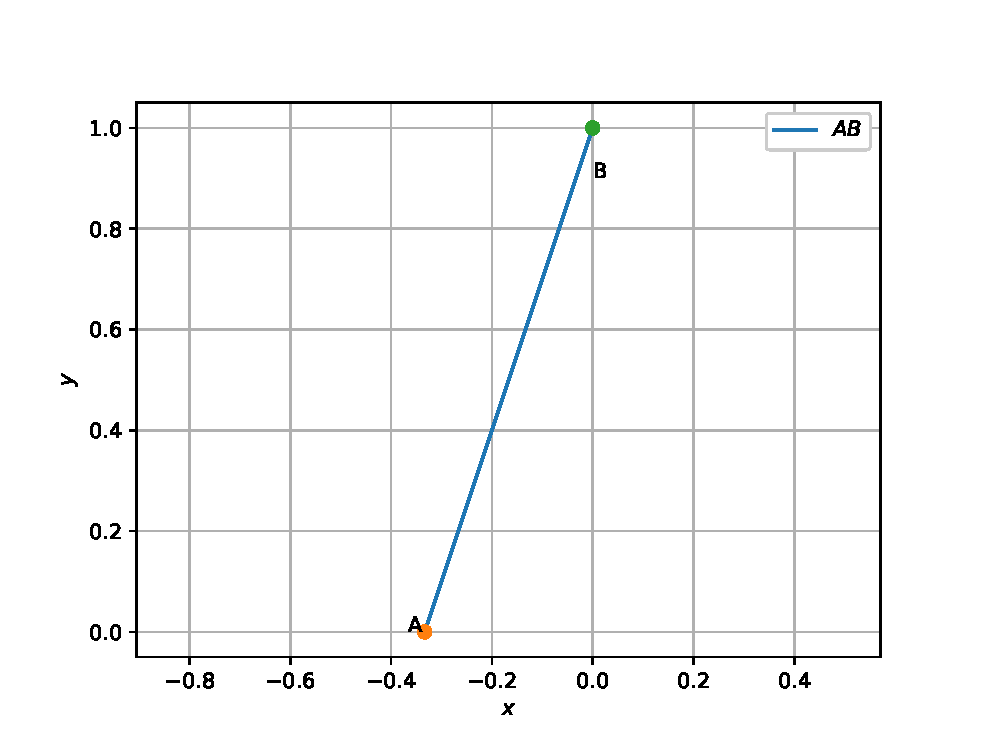
\includegraphics[width=\columnwidth]{./figs/line/line1.eps}
\caption{}
\label{fig:line1}
\end{figure}

\item Let 
%
\begin{align}
y &= 5x -\pi
\implies \myvec{5 & -1}\vec{x} &= \pi
\end{align}
%
Thus, 
%
\begin{align}
y &= 0 
\\
\implies  5x - \pi &=0
\\
\text{or, } x &= \frac{\pi}{5}
\end{align}
%
Hence $\vec{x}=\frac{4}{5}$ is not a zero. This is verified in Fig. \ref{fig:line2}.
%
\begin{figure}[!ht]
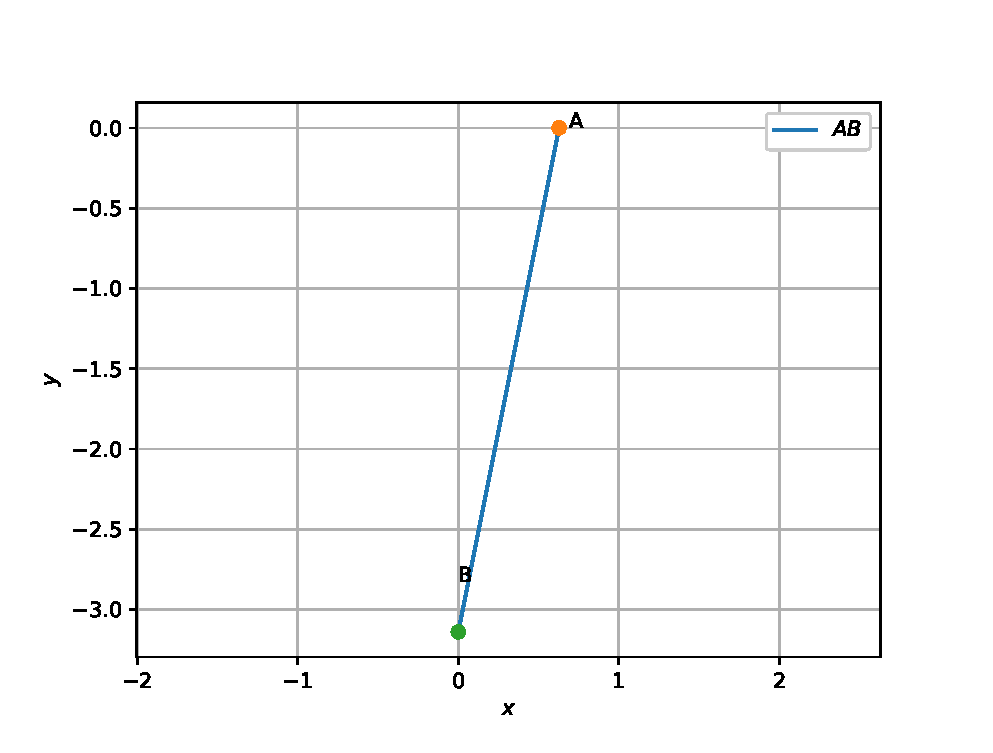
\includegraphics[width=\columnwidth]{./figs/line/line2.eps}
\caption{}
\label{fig:line2}
\end{figure}
\item Let 
%
\begin{align}
y &= 5lx + m
\implies \myvec{5l & -1}\vec{x} &= -m
\end{align}
%
Thus, 
%
\begin{align}
y &= 0 
\\
\implies  5lx + m &=0
\\
\text{or, } x &= -\frac{m}{5l}
\end{align}
%
Hence $\vec{x}=-\frac{m}{l}$ is not a zero. This is verified in Fig. \ref{fig:line3}.
%
\begin{figure}[!ht]
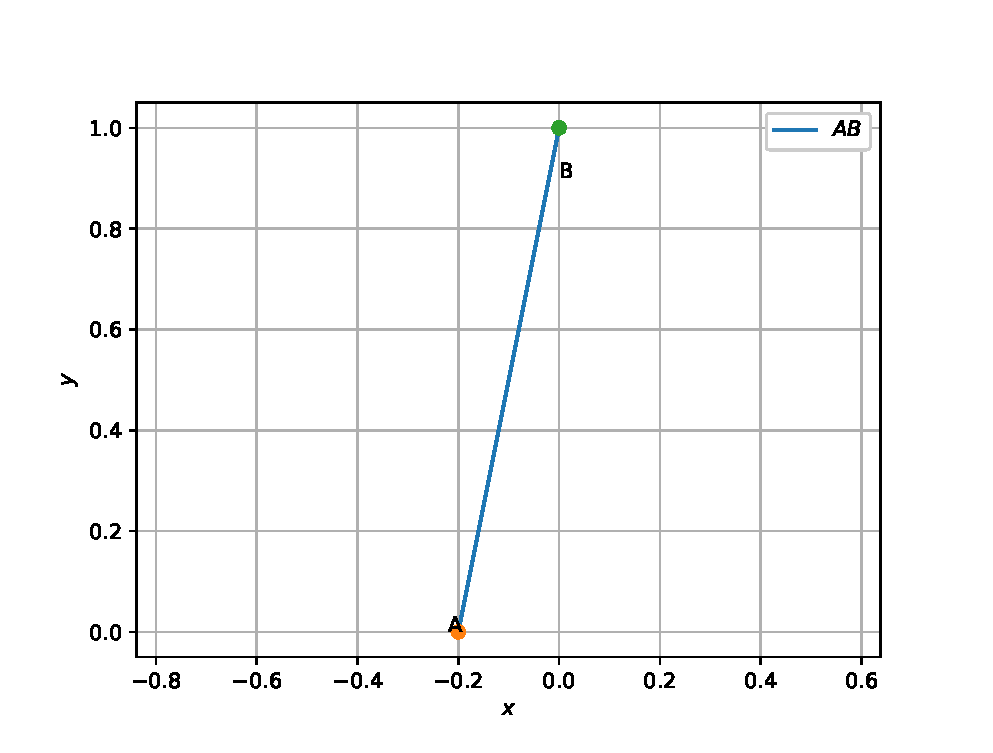
\includegraphics[width=\columnwidth]{./figs/line/line3.eps}
\caption{}
\label{fig:line3}
\end{figure}
\item Let 
%
\begin{align}
y &= 2x + 1
\implies \myvec{2 & -1}\vec{x} &= -1
\end{align}
%
Thus, 
%
\begin{align}
y &= 0 
\\
\implies  2x + 1 &=0
\\
\text{or, } x &= -\frac{1}{2}
\end{align}
%
Hence $\vec{x}=\frac{1}{2}$ is not a zero. This is verified in Fig. \ref{fig:line4}.
%
\begin{figure}[!ht]
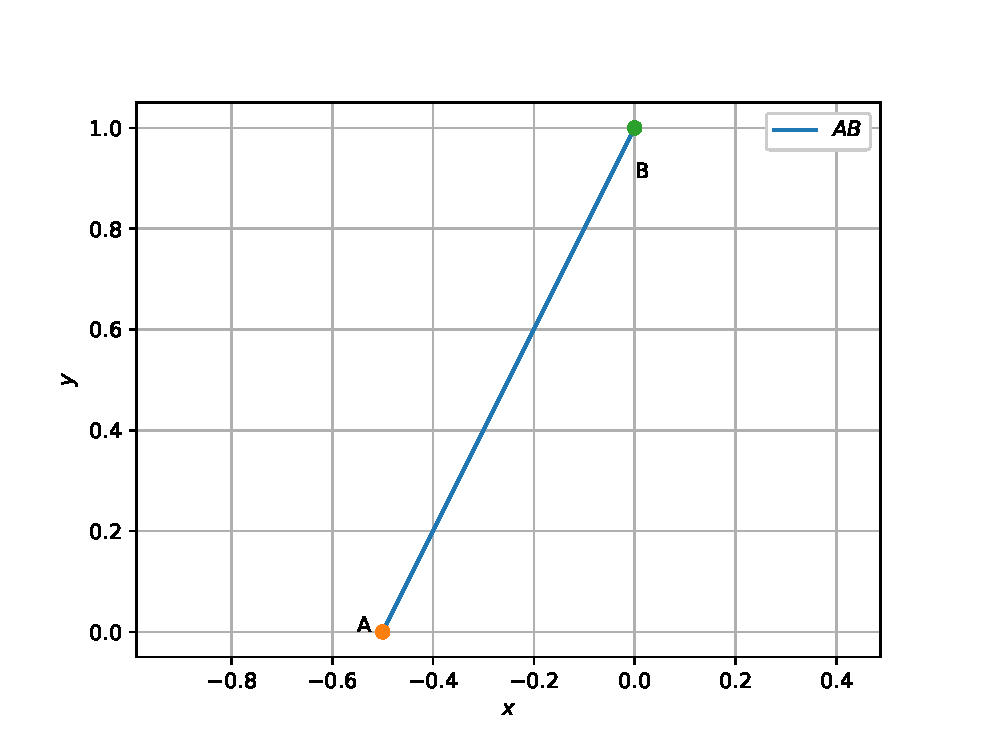
\includegraphics[width=\columnwidth]{./figs/line/line4.eps}
\caption{}
\label{fig:line4}
\end{figure}
\end{enumerate}